% --------------------------------------------------------------
% This is all preamble stuff that you don't have to worry about.
% Head down to where it says "Start here"
% --------------------------------------------------------------
 
\documentclass[12pt]{article}
 
\usepackage[margin=1in]{geometry} 
\usepackage{amsmath,amsthm,amssymb}
\usepackage{braket}
\usepackage{graphicx}
\usepackage{calligra}
\usepackage{calrsfs}
\usepackage{subcaption}
\usepackage{listings}
\newcommand{\N}{\mathbb{N}}
\newcommand{\Z}{\mathbb{Z}}
 
\newenvironment{theorem}[2][Theorem]{\begin{trivlist}
\item[\hskip \labelsep {\bfseries #1}\hskip \labelsep {\bfseries #2.}]}{\end{trivlist}}
\newenvironment{lemma}[2][Lemma]{\begin{trivlist}
\item[\hskip \labelsep {\bfseries #1}\hskip \labelsep {\bfseries #2.}]}{\end{trivlist}}
\newenvironment{exercise}[2][Exercise]{\begin{trivlist}
\item[\hskip \labelsep {\bfseries #1}\hskip \labelsep {\bfseries #2.}]}{\end{trivlist}}
\newenvironment{reflection}[2][Reflection]{\begin{trivlist}
\item[\hskip \labelsep {\bfseries #1}\hskip \labelsep {\bfseries #2.}]}{\end{trivlist}}
\newenvironment{proposition}[2][Proposition]{\begin{trivlist}
\item[\hskip \labelsep {\bfseries #1}\hskip \labelsep {\bfseries #2.}]}{\end{trivlist}}
\newenvironment{corollary}[2][Corollary]{\begin{trivlist}
\item[\hskip \labelsep {\bfseries #1}\hskip \labelsep {\bfseries #2.}]}{\end{trivlist}}
 
\begin{document}
 
% --------------------------------------------------------------
%                         Start here
% --------------------------------------------------------------
 
%\renewcommand{\qedsymbol}{\filledbox}
 
\title{HW5}
\author{Carl Mueller\\ %replace with your name
CSCI 5254 - Convex Optimization} %if necessary, replace with your course title
\maketitle

\subsection*{6.1}
\begin{proposition}{1}
\begin{align}
log(x+1) \le x\\ -log(x+1) \ge x\\ x > -1
\end{align}
\end{proposition}

\begin{proposition}{2}
\begin{align}
-log(1-x)\ \text{is convex}
\end{align}
\end{proposition}
\begin{proposition}{3}
\begin{align}
\phi(||u||_{\infty}) = -a^2log(1-\frac{||u||_{\infty}}{a^2})
\end{align}
\end{proposition}

Left inequality working backwards:
\begin{equation*}
\begin{aligned}
||u||_{2}^{2} \le -a^2\sum_{i=1}^{m}log(1 - \frac{u_{i}^{2}}{a^2})\\
\sum_{i=1}^{m}\frac{|u_i|^2}{a^2} \le -\sum_{i=1}^{m}log(1 - \frac{u_{i}^{2}}{a^2})\\
\end{aligned}
\end{equation*}
Given proposition 1:
\begin{equation*}
\begin{aligned}
\sum_{i=1}^{m}\frac{|u_i|^2}{a^2} \le -\sum_{i=1}^{m}log(1 - \frac{u_{i}^{2}}{a^2})\\
\text{true when: }\\
- \frac{u_{i}^{2}}{a^2} \ge -1
\end{aligned}
\end{equation*}

Right inequality:
\begin{equation*}
\begin{aligned}
\text{Given: } u_{i}^{2} \le ||u_i||_{\infty}^{2}\\
\sum_{i=1}^{m}-log(1 - \frac{u_{i}^{2}}{a^2}) \le \sum_{i=1}^{m}-log(1 - \frac{||u_{i}||_{\infty}^{2}}{a^2})\ \text{given proposition 1}\\
\sum_{i=1}^{m}-log(1 - \frac{u_{i}^{2}}{a^2}) \le \frac{u_{i}^{2}}{||u||_{2}^{\infty}}\sum_{i=1}^{m}-log(1 - \frac{||u_{i}||_{\infty}^{2}}{a^2})\ \text{given $\frac{u_{i}^{2}}{||u||_{2}^{\infty}} \ge 1$}\\
-a^2\sum_{i=1}^{m}log(1 - \frac{u_{i}^{2}}{a^2}) \le -a^2\frac{u_{i}^{2}}{||u||_{2}^{\infty}}\sum_{i=1}^{m}log(1 - \frac{||u_{i}||_{\infty}^{2}}{a^2})\\
-a^2\sum_{i=1}^{m}log(1 - \frac{u_{i}^{2}}{a^2}) \le \frac{u_{i}^{2}}{||u||_{2}^{\infty}}\phi(||u||_{\infty})\\
\end{aligned}
\end{equation*}

\subsection*{6.9}
To show convexity, the following level set must be convex:

$$S_{\alpha} = \set{t_i| \max_{i=1,\dots,k}|\frac{p(t_i)}{q(t_i)} - y_i| \le \alpha}$$

Due to absolute value, following inequalities must hold:
\begin{equation*}
\begin{aligned}
-\alpha q(t_i) \le y_i q(t_i)-p(t_i) \le \alpha q(t_i)
\end{aligned}
\end{equation*}
 This is represent two inequalities that define a polyhedron and is therefore convex. Since the level set is convex,
 the original minimzation problem is at least quasiconvex.

\subsection*{7.3}

\begin{proposition}{1}
\begin{align}
P(x|y=1) = \frac{1}{\sqrt{2 \pi}}\int_{x}^{\infty}e^{\frac{-z^2}{2}}dz\\
P(x|y=0) = 1 - \frac{1}{\sqrt{2 \pi}}\int_{x}^{\infty}e^{\frac{-z^2}{2}}dz
\end{align}
\end{proposition}

Ordering probability terms in order of $y=1$ and $y=0$, our total probability is:
\begin{equation*}
\begin{aligned}
p(a,b) = \prod_{i=1}^{q}P_i(a^Tu_i+b|y=1)\prod_{i=q+1}^{m}(1-P_i(a^Tu_i+b|y=0))\\
\end{aligned}
\end{equation*}
The negative log likelihood:
\begin{equation*}
\begin{aligned}
l(a,b) = \sum_{i=1}^{q}-log(P_i(a^Tu_i+b|y=1))+\sum_{i=q+1}^{m}-log(1-P_i(a^Tu_i+b|y=0))
\end{aligned}
\end{equation*}
The negative log likelihood is a convex function, so minimizing this function is a convex optimization problem.

\subsection*{7.4}
\subsubsection*{a)}
\begin{proposition}{1}
\begin{align}
\text{Sample mean: }
u = \frac{1}{N}\sum_{k=1}^{N}y_k\\
\text{Covariance: }
Y = \frac{1}{N}\sum_{k=1}^{N}(y_k-u)(y_k-u)^T
\end{align}
\end{proposition}

\begin{equation*}
\begin{aligned}
-\frac{N}{2}nlog(2\pi)-\frac{N}{2}log(det(R))- \frac{1}{2}R^{-1}\sum_{k=1}^{N}(y_k-a)(y_k-a)^T\\
= -\frac{N}{2}nlog(2\pi)-\frac{N}{2}log(det(R))- \frac{1}{2}R^{-1}\sum_{k=1}^{N}(y_ky_k^T-ay_k^T-y_ka^T+aa^T)\\
= -\frac{N}{2}nlog(2\pi)-\frac{N}{2}log(det(R))- \frac{1}{2}R^{-1}(\sum_{k=1}^{N}y_ky_k^T-\sum_{k=1}^{N}ay_k^T-\sum_{k=1}^{N}y_ka^T+\sum_{k=1}^{N}aa^T))\\
= -\frac{N}{2}nlog(2\pi)-\frac{N}{2}log(det(R))- \frac{1}{2}R^{-1}(\sum_{k=1}^{N}y_ky_k^T-\sum_{k=1}^{N}ay_k^T-\sum_{k=1}^{N}y_ka^T+Naa^T)\\
\end{aligned}
\end{equation*}

Substitute sample mean:
\begin{equation*}
\begin{aligned}
= -\frac{N}{2}nlog(2\pi)-\frac{N}{2}log(det(R))- \frac{1}{2}R^{-1}\sum_{k=1}^{N}y_ky_k^T-Nay^T-Nua^T+Naa^T\\
= R^{-1}\sum_{k=1}^{N}(y_k-a)(y_k-a)^T-R^{-1}N(a-u)(a-u)^T\\
= -\frac{N}{2}nlog(2\pi)-\frac{N}{2}log(det(R))- \frac{1}{2}(NR^{-1}Y + R^{-1}N(a-u)(a-u)^T)\\
= -\frac{N}{2}nlog(2\pi)-\frac{N}{2}log(det(R))- \frac{1}{2}(Ntr(R^{-1}Y) + N(a-u)R^{-1}(a-u)^T)
\end{aligned}
\end{equation*}

Set the gradient to zero to see $a$ and $R$ optimal values.
\begin{equation*}
\begin{aligned}
\nabla_a l(R,a) = -2R^{-1}(a-u) = 0\\
\therefore a=u \\
\nabla_R l(R,a) = -R^{-1} + R^{-1}(Y - (a-u)(a-u)^T)R^{-1} = 0\\
R = Y + (a-u)(a-u)^T\\
R = Y + (0)(0)^T\\
\therefore R=Y
\end{aligned}
\end{equation*}

\subsection*{7.8}

Express sign function as a probability where we order values with $y>1$ followed by $y<0$:
\begin{equation*}
\begin{aligned}
\prod_{i=1}^{k}prob(a_i^Tx + b_i + v_i > 0)\prod_{i=k+1}^{m}prob(a_i^Tx + b_i + v_i < 0)
\end{aligned}
\end{equation*}

Since $a_i$ and $b_i$ are known values, the only RV is the noise term. We can epxress $v_i$ as an expression of $a_i^Tx+b_i$. P represents the cumulative density function of $v_i$. We can represent the probability as follows:
\begin{equation*}
\begin{aligned}
\prod_{i=1}^{k}P(-a_i^Tx-b_i)\prod_{i=k+1}^{m}1-P(-a_i^Tx-b_i) 
\end{aligned}
\end{equation*}

Log likelihood below is concave so if we maximize, we obtain a convex problem:
\begin{equation*}
\begin{aligned}
l(x) = \sum_{i=1}^{k}log(P(-a_i^Tx-b_i))+\sum_{i=k+1}^{m}log(1-P(-a_i^Tx-b_i))\\ 
\end{aligned}
\end{equation*}

\subsection*{7.9}
Given $$y_i = f(a_i^Tx +b_i +v_i), i=1,\dots,m$$
We know that $a_i$ and $b_i$ are knowns, so lets expression the random variable $v_i$ as an expression of all other terms. We assume that $f$ is an invertible function.
$$v_i = f^{-1}(y_i)-a_i^Tx-b_i$$
The probability of observing $y_i,\dots,y_m$ is:
\begin{equation*}
\begin{aligned}
\prod_{i=1}^{m}prob(f^{-1}(y_i)-a_i^Tx-b_i)\\
l(x, f) = \sum_{i=1}^{m}log(prob(f^{-1}(y_i)-a_i^Tx-b_i))
\end{aligned}
\end{equation*}
This log probability is concave w.r.t x and f. Thus maximizing generates a convex optimization problem.\\\\

\textbf{Additional Exercises:}\\\\
\subsection*{3.9}
\subsubsection*{a)}
Given: $$z = [\Re x, \Im x]$$

Setup a system of equations using the vector breakdown of x for its $\Re$ and $\Im$ components:
\begin{equation*}
\begin{aligned}
||x||_2^2 = ||z||_2^2\\
\begin{bmatrix}
\Re A & -\Im A\\
\Im A & \Re A
\end{bmatrix}
\begin{bmatrix}
\Re x \\
\Im x
\end{bmatrix}=
\begin{bmatrix}
\Re b\\
\Im b
\end{bmatrix}
\end{aligned}
\end{equation*}

This becomes the optimization problem:
\begin{equation*}
\begin{aligned}
& \underset{z}{\text{minimize}}
& & ||z||_2\\
& \text{subject to}\
& &
\begin{bmatrix}
\Re A & -\Im A\\
\Im A & \Re A
\end{bmatrix}
\begin{bmatrix}
\Re x \\
\Im x
\end{bmatrix}=
\begin{bmatrix}
\Re b\\
\Im b
\end{bmatrix}
\end{aligned}
\end{equation*}

\subsubsection*{b)}
Define the second order cone:
\begin{equation*}
\begin{aligned}
K_i = \set{(z,t)| ||z||_2 \le t}
\end{aligned}
\end{equation*}
The SOCP:
\begin{equation*}
\begin{aligned}
& \underset{}{\text{minimize}}
& & t\\
& \text{subject to}\
& |z||_2\\
& &
\begin{bmatrix}
\Re A & -\Im A\\
\Im A & \Re A
\end{bmatrix}
\begin{bmatrix}
\Re x \\
\Im x
\end{bmatrix}=
\begin{bmatrix}
\Re b\\
\Im b
\end{bmatrix}\end{aligned}
\end{equation*}
\subsubsection*{c)}
\textbf{Code:}
\begin{lstlisting}
randn('state',0);
m = 30; n = 100;
Are = randn(m,n); Aim = randn(m,n);
bre = randn(m,1); bim = randn(m,1);
A = Are + i*Aim;
b = bre + i*bim;

Atot = [Are -Aim; Aim Are];
btot = [bre; bim];
z_2 = Atot'*inv(Atot*Atot')*btot;
x_2 = z_2(1:100) + i*z_2(101:200);

cvx_begin
    variable x(n) complex
    minimize( norm(x) )
    subject to
    A*x == b;
cvx_end

cvx_begin
    variable xinf(n) complex
    minimize( norm(xinf,Inf) )
    subject to
    A*xinf == b;
cvx_end

figure(1)
scatter(real(x),imag(x)), hold on,
scatter(real(xinf),imag(xinf),[],'filled'), hold off,
axis([-0.2 0.2 -0.2 0.2]), axis square,
xlabel('Re x'); ylabel('Im x');
\end{lstlisting}
Results:
\begin{figure}[h]
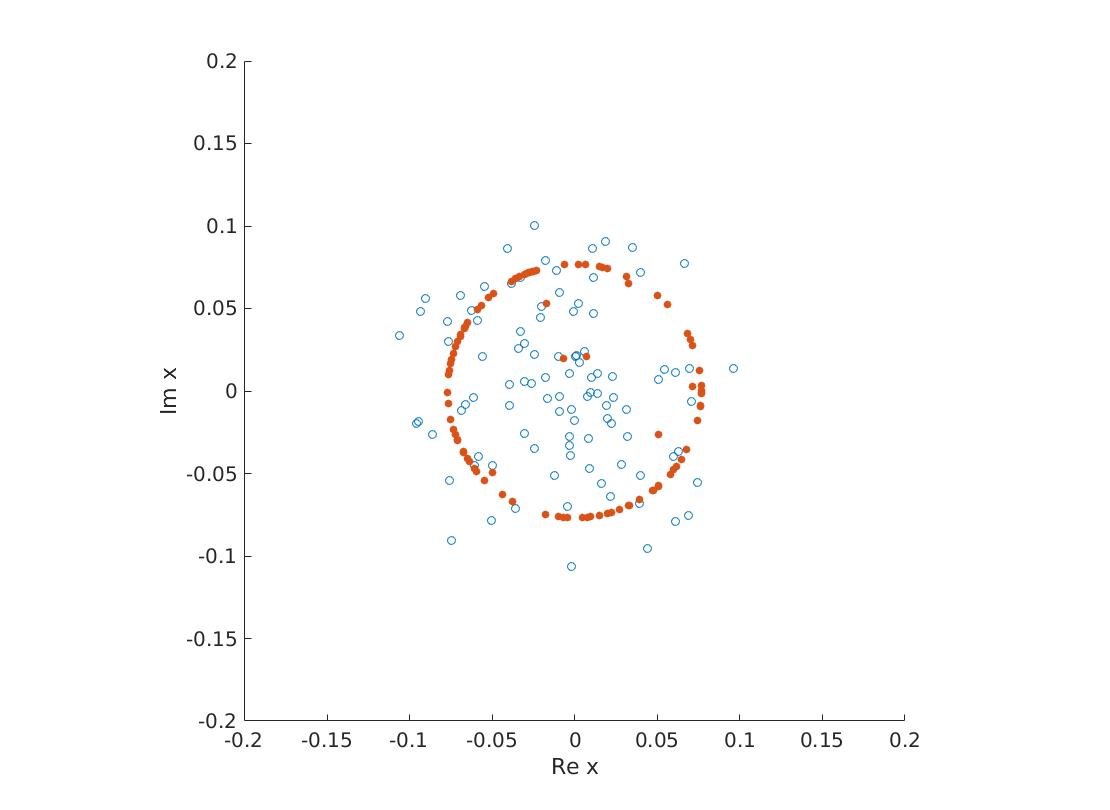
\includegraphics[scale=.25]{39c.jpg}
\end{figure}
The red dots represent the infinity norm.

\subsection*{4.1}
\subsubsection*{a)}
Code:
\begin{lstlisting}
M = [1 -1/2; -1/2 2];
m = [-1 0]';
A = [1 2; 1 -4; 5 76];
b = [-2 -3 1]';
delta = .1

cvx_begin
    variable x(2)
    dual variable y
    minimize(quad_form(x, M)+m'*x)
    subject to
        y: A*x <= b;
cvx_end
p_star = cvx_optval
y
x
\end{lstlisting}
\textbf{Results:}\\
p\_star = 8.2222\\
y = \\1.8994\\
    3.4684\\
    0.0931\\
x =\\-2.3333\\
    0.1667\\\\
\underline{KKT Conditions}\\
Primal:\\
$$x_1^* + 2x_2^* \le u_1$$
$$x_1^* + -4x_2^* \le u_2$$
$$5x_1^* + 76x_2^*\le 1$$
Dual:\\
$$\lambda_1^*, \lambda_2^*, \lambda_3^* \ge 0$$
Complementary Slackness:
$$\lambda_1^*(x_1^* + 2x_2^* - u_1)=0$$
$$\lambda_2^*(x_1^* + -4x_2^* - u_2)=0$$
$$\lambda_3^*(5x_1^* + 76x_2^* - 1)=0$$
First Order Conditions:
$$4x_2^*-x_1^*+2\lambda_1^*-4\lambda_2^*+76\lambda_3^*=0$$
$$2x_1^* -x_2^*-1+\lambda_1^*+\lambda_2^*+5\lambda_2^*=0$$
\subsubsection*{b)}
\textbf{Code:}
\begin{lstlisting}
M = [1 -1/2; -1/2 2];
m = [-1 0]';
A = [1 2; 1 -4; 5 76];
b = [-2 -3 1]';

cvx_begin
    variable x(2)
    dual variable y
    minimize(quad_form(x, M)+m'*x)
    subject to
        y: A*x <= b;
cvx_end
p_star = cvx_optval

array = [0 -1 1];
table = [];
delta = 0.1;

for i = array
    for j = array
        p_pred = p_star - [y(1) y(2)]*[i; j]*delta;
        cvx_begin
            variable x(2)
            minimize(quad_form(x,M)+m'*x)
            subject to
                A*x <= b+[i;j;0]*delta
        cvx_end
        p_exact = cvx_optval;
        table = [table; i*delta j*delta p_pred p_exact]
    end
end
\end{lstlisting}
\textbf{Results:}
\begin{center}
  \begin{tabular}{ | c | c | c | c |}
  \hline
    d_1 & d_2 & p^*_{pred} & p^*_{exact} \\ \hline
    0 &        0  &  8.2222  &  8.2222 \\ \hline
    0&   -0.1000    &8.5691   & 8.7064 \\ \hline
    0    &0.1000    &7.8754    &7.9800 \\ \hline
    -0.1000&         0 &   8.4122 &    8.5650 \\ \hline
    -0.1000&   -0.1000  &  8.7590  &  8.8156 \\ \hline
    -0.1000&    0.1000  &  8.0653  &  8.3189 \\ \hline
    0.1000 &        0   & 8.0323   & 8.2222 \\ \hline
    0.1000 &  -0.1000    &8.3791   & 8.7064 \\ \hline
    0.1000 &   0.1000   & 7.6854   & 7.7515 \\ \hline
  \end{tabular}
\end{center}
We can see that $p^*_{pred} \le p^*_{exact}$ for all pertubations.



% --------------------------------------------------------------
%     You don't have to mess with anything below this line.
% --------------------------------------------------------------
 
\end{document}